% INTRODUCTION CHAPTER LAYOUT
%
% 1. Problem Statement: Introduce readers to the topic
%  What is the "problem"
%  Brief summary of current solution and why it is inadaquate (if applicable)
%  Why the research is worth tackling, why a solution would be significant
%
% 2. Aim: State overall research aim (try for 1 sentence)
%  Several developments / stages will be required in any research to produce a final
%    result, however remember that only the final outcome is the aim, not each stage
%    i.e. tell the reader what the aim is, not how you are going to achieve it. You
%    will explain this in more specific chapters.
%  There should only be 1 aim
%  The aim should follow as a logical consequence of the problem statement
%  You should be able to relate to this aim throughout the thesis, particularly conclusion
%  "Thus ..."
%
% 3. Scope: State scope of work
%  Be very clear what will and will not be covered. Justify why. 
%  It is okay to have persued only one of multiple accepted approaches due to limited time, 
%    but justify why you have chosen this approach over another.
%  If you want sections in this chapter, Aim & Scope can be together
%
% 4. Overview of the study: Brief chapter layout & description of work to come
%  "To achieve this Chapter ..."
%  Similar to the table of contents, but you are explaining the logical flow of 
%    your thesis to ensure the reader can see where you are going and why
%  By the end of this section the reader should understand how the aim will be
%    achieved.
%
% Do NOT include:
%  - review of literature
%  - statement of theory
%  - glossary of terms (although sometimes it is important to define terms when defining
%      the scope of your work)
%
% Most of this info is summarised from the book below. Supervisors may have other preferences,
% but I found it very helpful. I've only included short summaries in this template but if you
% are stuck buying a copy is definitely worth it :) http://www.mup.com.au/items/120101
%  Evans, D., Gruba, P. & Zobel, J., 2011. How to Write a Better Thesis, Melbourne University Press.

\chapter{Introduction}
\label{cha:introduction}

\section{Background}
\label{sec:intro_background}

Needed:
-Place in industry
-Background of diagnosis
-Requirement and fit in company
-Existing equiptment

Within the healthcare industry, there is a continuous need for fast and reliable diagnostics of pathogens within patients. Identifying the presence of pathogens responsible for disease in a patient allows the appropriate preventive or corrective action to be taken and represents a crucial step in treating or preventing illness. This thesis was conducted for the benefit of and in collaboration with AusDiagnostics Pty Ltd.\\

Successful diagnostics, within the context of this thesis, can be summarised in three overall stages. Namely these are extraction, amplification and finally analysis. This thesis concerns itself only with extraction. It should be noted that not all pathogen analysis and/or commercial diagnostic processes follow these steps strictly, however the processes and technologies applied by AusDiagnostics follow this procedure. The stages of this procedure may be summarised as follows:
\begin{enumerate}
	\item [1. Extraction] To begin the diagnosis, a clinical sample is obtained from the patient. This sample may consist of cerebrospinal fluid, faecal matter, urine or others, depending on the disease to be diagnosed. These samples contain the target DNA or RNA which will later be analysed to determine the presence of the pathogen and hence disease. They also contain however a number of inhibitors to the process of amplification and analysis. Extraction is the process of removing said inhibitors and retaining only the target DNA or RNA. The result is refered to as a clean sample.
	\item  [2. Amplifcation] Amplification takes the clean sample and by one of many methods increases the overall count of the DNA. This may be with the intention of allowing multiple targets to be detected or to increase the sensitivity of the analysis.
	\item[3. Analysis] Analysis uses one of many available methods to search for the presence of biomarkers within the amplified clean sample. The presence of the biomarker indicates the result of the diagnosis.
\end{enumerate}

AusDiagnostics currently supplies customers with the instruments and chemical products required to complete stages two and three (amplification and analysis) of the diagnosis. This requires customers to purchase extraction equipment from alternative suppliers and represents a significant weakness and loss of profit. Research and development conducted by AusDiagnostics has determined that the optimal approach, when considering speed and efficiency, is super-paramagnetic bead based extraction. The beads utilised are of the shell-core variety. The core is composed of an iron oxide, which provides the super paramagnetic properties required for physical manipulation of the beads via a magnetic field. The shell is comprised of silica, which via chemical modification has the propensity to bond DNA and RNA to the bead surface. The techniques developed by researchers at AusDiagnostics utilising the magnetic silica beads have been validated and verified via manual operation. This thesis concerns itself with the automation of the developed extraction process, to produce a commercially viable robotic instrument. This instrument will be referred to as the Gene-Plex Extractor.\\

The extraction process to be automated has a number of notable requirements. These include liquid handling via precise pipetting, including mixing and liquid transfer. Also required is manipulation of the magnetic silica beads to separate the bonded and hence captured target DNA or RNA, along with heating to a specified, constant temperature to act to increase the rate of the chemical processes. The automation of the extraction process will be achieved by integrating the required capabilities into the robot produced by AusDiagnostics to conduct the amplification stage of diagnosis. The instrument, based of the Gene-Plex platform and sold as the High-Plex Processor, is pictured in it's current application in Figure \ref{fig:highplex}. The Gene-Plex platform is essentially a liquid handling robot. The robot carries out the amplification stage by precisely pipetting and transferring liquid mixtures between the tubes and instruments on the deck, using disposable tips. Each individual assay (an analysis conducted to determine the presence and amount of a substance within a volume) utilises an individual layout of components on the robots deck. This makes the platform highly configurable for differing setups.\\

\begin{figure}
	\centering
	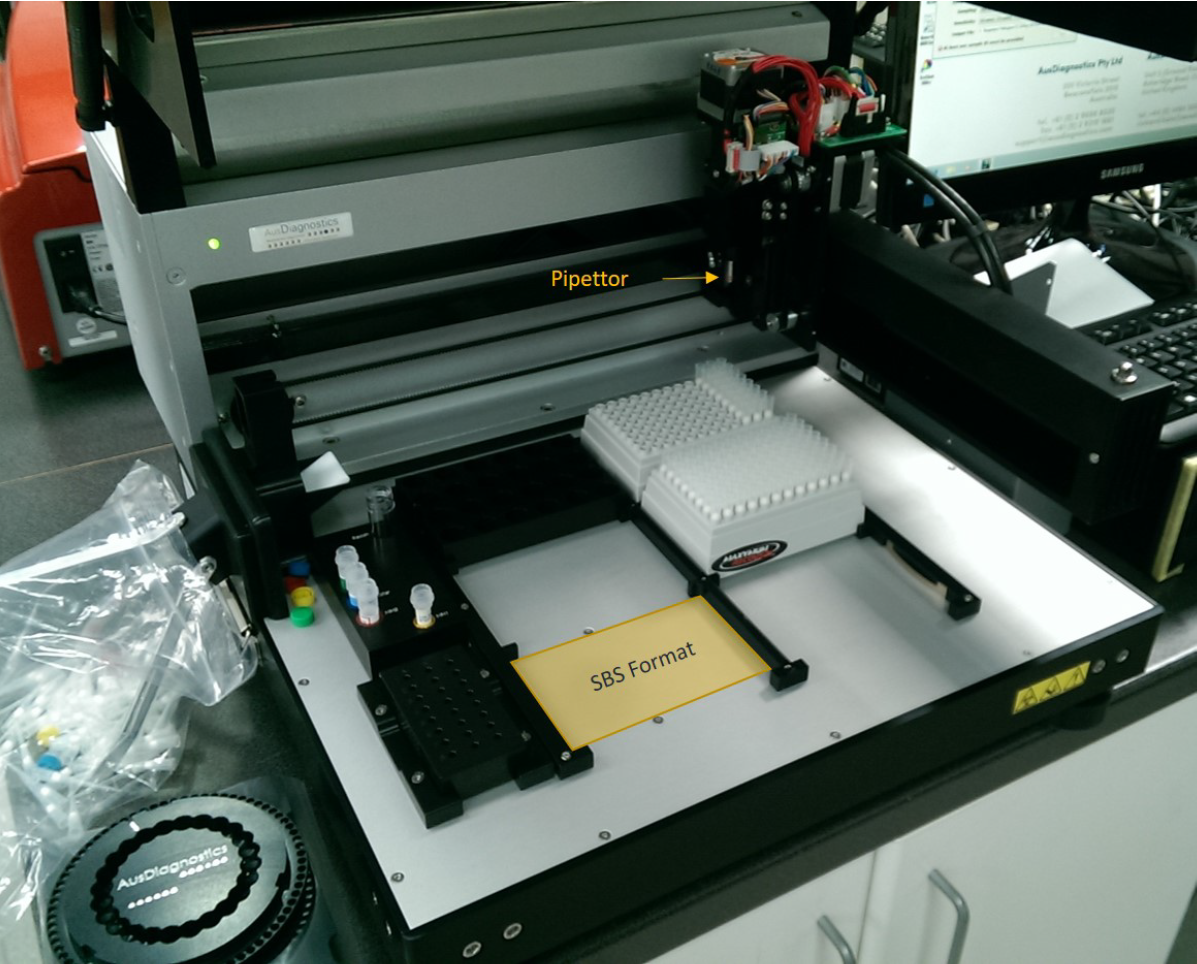
\includegraphics{highplex.png}
	\caption[High-Plex Platform.]{The Gene-Plex liquid handling robot platform, as implemented as the High-Plex Processor.}
	\label{fig:highplex}
\end{figure}ˆ 

\subsection{The Extraction Process}
\label{subsec:intro_extraction}

In order to allow the aim and scope of the work to be clearly defined, a condensed overview of the extraction process developed by AusDiagnostics is presented. It should be noted that unless explicitly stated, all operations are to be automated.\\

The extraction process requires that the clinical sample undergoes a number of chemical steps across different locations on the robot. To aid in understanding the liquid handling involved, Figure \ref{fig:decklayout} displays the important sites on the deck. The process will begin with the operator manually loading 24 individual clinical samples into the location labelled ``Clinical Samples". In order to conform to existing products used by customers, it is then required that the chemical processing takes place in the locations labelled ``Samples". In order to transfer the liquid between locations, the robot will pick up 1000$\mu$L tips from the locations marked ``Tips".\\

The sample processing locations must accept modules that fit within the standard block size (SBS) format. These blocks are required to each accept 8 cassettes, one for each sample (pictured in Figure \ref{fig:cassette}). Each cassette includes 6 tubes, which will be the site of a particular chemical reaction in order to extract the target DNA and RNA:
\begin{enumerate}
	\item 500$\mu$L of clinical sample is pipetted into tube location 2, as marked in Figure \ref{fig:cassette}. Within this tube as supplied by AusDiagnostics, there will already be 10$\mu$L of magnetic bead mixture along with 440$\mu$L of lysis buffer. The lysis buffer will destroy the cell walls, releasing the target DNA or RNA to be bound to the magnetic silica beads. This process is required to take place at 60$\degree$C in order to increase the rate of reaction Due to the low volume of liquid in this step, it is to be completed in one of the 1mL low profile tubes. This aids with liquid handling precision.
	\item The target DNA or RNA is now bound to the beads, which are suspended in the waste liquid (supernatant). In order to capture only the bead suspension, the entire liquid mixture is aspirated via pipette tip and subsequently move to the location marked ``Waste Separation". In this location, a magnetic field is to be applied to capture the magnetic silica beads within the pipette tip. While captured, the supernatant must then be expelled into a waste container in this location. The tip now contains only the magnetic beads with bound targets.
	\item Despite the supernatant having been expelled, there will still be a significant amount of waste retained on the bead surface. To remove this and clean the beads, a sequence of 3 wash steps must then occur in tube locations 1, 5 and 6. To achieve this, the beads are first re-suspended in the tube, which contains 800$\mu$L of a particular wash buffer. The suspension must then be mixed via pipetting in order to to ensure the bead surface is properly exposed. The entire liquid mixture is then aspirated once again and transferred to the waste location, where via the same means as step 2, the waste liquid is disposed of while the beads are retained. This process is repeated 3 times in the tubes noted above to ensure no waste matter clings to the bead surface.
	\item With the beads now clean and still bound to the target, the mixture is transferred to location 3 of the cassette. The elution buffer is used to break the bond between the target DNA and RNA and the magnetic silica beads. This process is also required to be completed at 60$\degree$C to reduce the time required. Following this step, the target DNA or RNA of interest is now contained within the elution buffer, along with the magnetic silica beads which are now waste.
	\item The final step is to capture only the target DNA or RNA within the elution buffer, leaving behind the magnetic beads. This is required to take place in tube location 4. This is a low volume reaction, containing only 100$\mu$L of elution buffer and is therefore completed in the final small profile tube. The pipette must then aspirate this mixture, following bead removal, and contain only the elution buffer and target mixture required for amplification in stage 2 of the assay.
\end{enumerate}

\begin{figure}
	\centering
	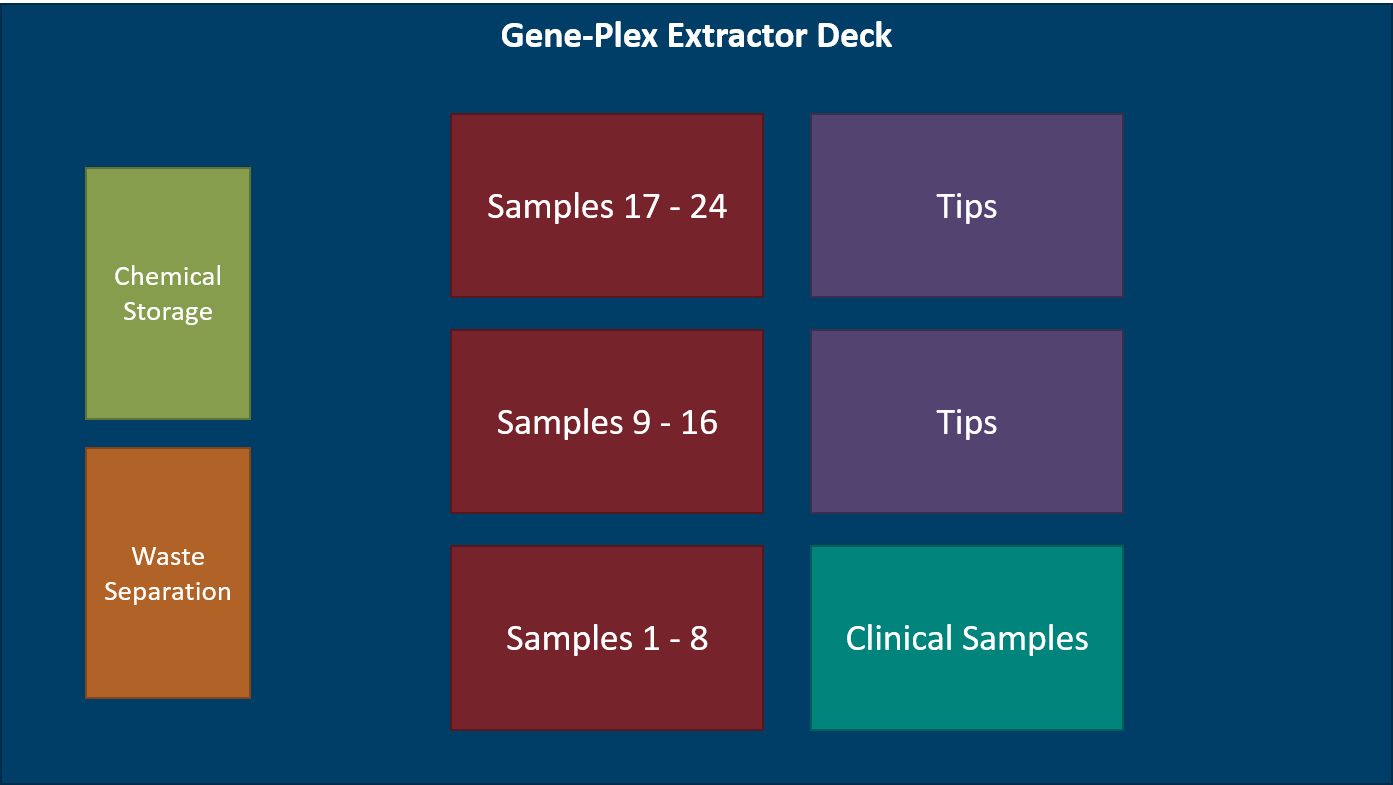
\includegraphics{decklayout.png}
	\caption[Extractor deck layout.]{The layout to be used for the Gene-Plex Extractor.}
	\label{fig:decklayout}
\end{figure}ˆ 

\begin{figure}
	\centering
	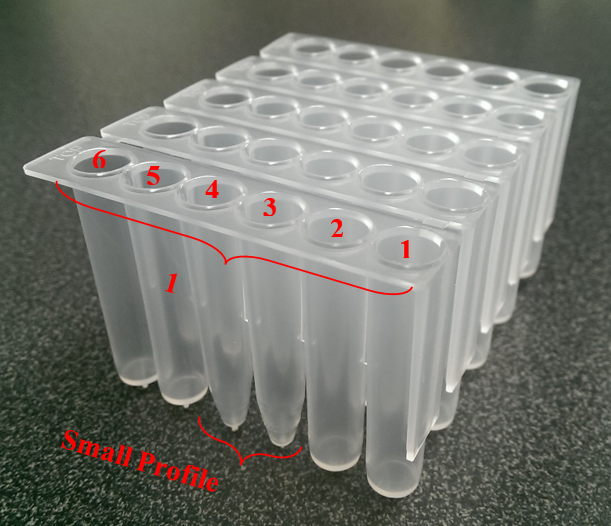
\includegraphics{cassette.png}
	\caption[Extraction cassette tubes.]{The tube format to be used as the site of the sample processing.}
	\label{fig:cassette}
\end{figure}ˆ 


\section{Aim}
\label{sec:intro_aim}
%May bee to summarise what is missing from the robot before stating the aim
This work aims to develop and integrate into the Gene-Plex Robot Platform the hardware necessary for carrying out the described chemical processes, the required magnetic manipulations and the controller necessary to maintain the stipulated constant 60$\degree$C temperature.\\

\section{Scope}
\label{sec:intro_scope}


\section{Methodology}
\label{sec:intro_method}




% Figure 1.1 is defined below (Large mechatronics logo). Note figures are placed automatically by LaTeX and will not necessarily be placed before the next text.
\begin{figure}
\centering

\includegraphics{mechatronicslogo2_no_UNSW.png}
\caption[Short caption for list of figures.]{Full caption for the Mechatronics Logo. Designed by Wei Hua Chen.}
\label{fig:intro_logo}
\end{figure}

\begin{figure}[!ht] \centering
\captionsetup[subfigure]{width=2.5in} % <-- Use this to control text which is poorly spaced under a subfigure. 
\begin{subfigure}[t]{0.45\textwidth}

\includegraphics[width=\textwidth]{mechatronicslogo2_no_UNSW.png}
\caption[Subfigure caption.]{Subfigure caption.}
\label{fig:intro_subfig1}
\end{subfigure}
\begin{subfigure}[t]{0.45\textwidth}

\includegraphics[width=0.5\textwidth]{mechatronicslogo2_no_UNSW.png}
\caption[Subfigure caption.]{Subfigure caption.}
\label{fig:intro_subfig2}
\end{subfigure}
\caption[Abbreviated caption.]{Overall figure caption.}
\label{fig:intro_subfig}
\end{figure}

Figure \ref{fig:intro_subfig} and subfigure \ref{fig:intro_subfig2} or \subref{fig:intro_subfig2} contains ...
Table \ref{tab:intro_table_1}. 

Citations: Luce \cite{luce_probabilistic_1958} wrote something important.

% Note: You can add a table of figures to the header pages by uncommenting \listoftables in the frontpages.tex

\begin{table}[h!]
\begin{center}
\begin{tabular}{ p{3cm}  p{4cm} | p{6.5cm} }
\hline
Classification & Cost & Description\\ \hline \hline
CLEAR & 1 & Good for traversing\\ \hline
OBSTACLES  & $\infty$ & Definitely not traversable\\ \hline
UNKNOWN & 4 if distant, $\infty$ if close & Not classified\\ \hline
EXPENSIVE & In range $[2, 50]$ & Traversable but should be avoided\\ \hline
\end{tabular}
\end{center}
\caption[Example table (short caption).]{Example table.}
\label{tab:intro_table_1}
\end{table}